\subsection{Pixel Drawing}

\begin{frame}{Accessing pixel data}
  \begin{itemize}
  \item Information required to access pixel data in memory:
    \begin{itemize}
    \item Pixel format (also modifier if not linear/raster order)
    \item Dimensions (and total size)
    \item Pointer to the base buffer address
    \end{itemize}
  \item The size of each line is called \textbf{stride} or \textbf{pitch}
    \begin{itemize}
    \item Usually equals: \(stride = width \times bpp \div 8\)
    \item Can contain an extra dead zone at the end
    \item Also needs to be specified explicitly
    \end{itemize}
  \item CPU access is either byte or word-aligned
    \begin{itemize}
    \item Good fit for formats with \(bpp = 32\) (very common)
    \item Good fit for formats with \(bpp = 8 \times n\)
    \item Not always easy to manage otherwise
    \end{itemize}
  \end{itemize}
\end{frame}

\begin{frame}[fragile]{Iterating over pixel data}
  \begin{itemize}
  \item Selected format (slides and demos): \textbf{XRGB8888}
    \begin{itemize}
    \item \(bpp = 32 = 8 \times 4\), one byte per channel, one memory plane
    \end{itemize}
  \item Pixel data can be access by iterating nested variables:
  \begin{minted}[fontsize=\small]{c}
for (y = 0; y < height; y++)
  for (x = 0; x < width; x++)
    data = base + y * stride + x * 4;
  \end{minted}
  \item Iterating over all pixels takes numerous CPU-cycles, tips:
    \begin{itemize}
    \item Incrementing the address instead of re-calculating it:
  \begin{minted}[fontsize=\small]{c}
data = base;
for (y = 0; y < height; y++)
  for (x = 0; x < width; x++)
    data += 4;
  data += stride - width * 4;
  \end{minted}
    \item Iterating in y-major is also better for cache hits
    \item Beware: C pointer arithmetic uses type size as unit
    \end{itemize}
  \end{itemize}
\end{frame}

\begin{frame}{Concepts about rasterization}
  \begin{itemize}
  \item Rasterization is the process of drawing vector shapes as discrete pixels
    \begin{itemize}
    \item Vector shapes are defined with mathematical equations
    \item Converted from a continuous space domain: \(\mathbb{R}^2\) to a discrete domain
    \item Results in a discretization/quantization error due to integer rounding
    \item Also subject to aliasing-related trouble
    \end{itemize}
  \end{itemize}
  \vspace{1em}
  \begin{minipage}[b]{0.45\textwidth}
    \centering
    \includegraphics[width=0.8\textwidth]{slides/graphics-theory-pixel-drawing/raster-source.jpg}
    \textit{\small Continuous source representation}
  \end{minipage}
  \hfill
  \begin{minipage}[b]{0.45\textwidth}
    \centering
    \includegraphics[width=0.8\textwidth]{slides/graphics-theory-pixel-drawing/raster-destination.jpg}
    \textit{\small Rasterized destination representation}
  \end{minipage}
\end{frame}

\begin{frame}{Rectangle drawing}
  \begin{itemize}
  \item A rectangle is defined with two boundaries per axis:
\[
x_{min} \leq x \leq x_{max},~ y_{min} \leq y \leq y_{max}
\]
  \item Another expression involves a (top-left) start point and size:
\[
x_{start} \leq x \leq x_{start} + x_{size},~ y_{start} \leq y \leq y_{start} + y_{size}
\]
  \item Allows iterating in the rectangle area only
  \end{itemize}
\end{frame}

\begin{frame}{Linear gradient drawing}
  \begin{itemize}
  \item Same base as drawing a rectangle
  \item A linear gradient involves interpolation between two colors
  \item Following one of the two axes as major
  \item Involves weighting the two colors depending on the advancement
  \item Equations in x-axis major:
  \end{itemize}
\begin{align*}
r &= r_{start} + (r_{stop} - r_{start}) \frac{x - x_{start}}{x_{size}}\\
g &= g_{start} + (g_{stop} - g_{start}) \frac{x - x_{start}}{x_{size}}\\
b &= b_{start} + (b_{stop} - b_{start}) \frac{x - x_{start}}{x_{size}}
\end{align*}
\end{frame}

\begin{frame}{Disk drawing}
  \begin{itemize}
  \item A disk is delimited with a radius test (\((0,0)\)-centered):
\[
\sqrt{x^2 + y^2} \leq radius
\]
  \item Given a center point \((x_c,y_c)\):
\[
\sqrt{(x - x_c)^2 + (y - y_c)^2} \leq radius
\]
  \item Requires iterating in:
\[
x_c - radius \leq x \leq x_c + radius,~ y_c - radius \leq y \leq y_c + radius
\]
  \end{itemize}
\end{frame}

\begin{frame}{Circular gradient drawing}
  \begin{itemize}
  \item Same base as drawing a disk
  \item Interpolation between two colors using the radius as major:
  \end{itemize}
\begin{align*}
d &= \sqrt{(x - x_c)^2 + (y - y_c)^2}\\
r &= r_{start} + (r_{stop} - r_{start}) \frac{d}{radius}\\
g &= g_{start} + (g_{stop} - g_{start}) \frac{d}{radius}\\
b &= b_{start} + (b_{stop} - b_{start}) \frac{d}{radius}
\end{align*}
\end{frame}

\begin{frame}{Line drawing}
  \begin{itemize}
  \item A line is defined as an affine function:
\[
y(x) = a \times x + b
\]
  \item Given start and end points, iterating in x-major:
\begin{gather*}
y(x) = y_{start} + (x - x_{start}) \times \frac{y_{end} - y_{start}}{x_{end} - x_{start}}\\
x_{start} \leq x \leq x_{stop}
\end{gather*}
  \item Axis major depends on the largest per-axis span (\(axis_{stop} - axis_{start}\))
    \begin{itemize}
    \item Iterating with smaller-span axis-major results in visual holes
    \item Iterating on both axes provides coherent results
    \end{itemize}
  \item Algorithms producing better-looking results:
    \begin{itemize}
    \item \textbf{Bresenham's} line algorithm, optimized for implementation
    \item \textbf{Xiaolin Wu's} line algorithm, with sub-pixel rendering
    \end{itemize}
  \end{itemize}
\end{frame}

\begin{frame}{Line and shape aliasing, sub-pixel drawing}
  \begin{itemize}
  \item Lines are often subject to aliasing:
    \begin{itemize}
    \item Sampled from the continuous domain with pixel sampling resolution
    \item Selecting the best axis gives a better resolution
    \item Limited display resolutions still make them look pixelated
    \end{itemize}
  \item Any geometric shape is affected, especially fonts
  \item Sub-pixel rendering is used to provide anti-aliased results:
    \begin{itemize}
    \item Surrounding pixels are given an intermediate value
    \item Specific algorithms perform sub-pixel drawing
    \item Also obtained with high-resolution rendering and anti-aliased downscaling
    \end{itemize}
  \end{itemize}

  \begin{center}
  \includegraphics[height=4em]{slides/graphics-theory-pixel-drawing/diamond-sub-pixel.png}
  \includegraphics[height=4em]{slides/graphics-theory-pixel-drawing/line-sub-pixel.png}\\
  \textit{\small Shapes rendered without and with sub-pixel anti-aliasing}
  \end{center}
\end{frame}

\begin{frame}{Line and shape aliasing, sub-pixel drawing (illustrated)}
  \begin{center}
  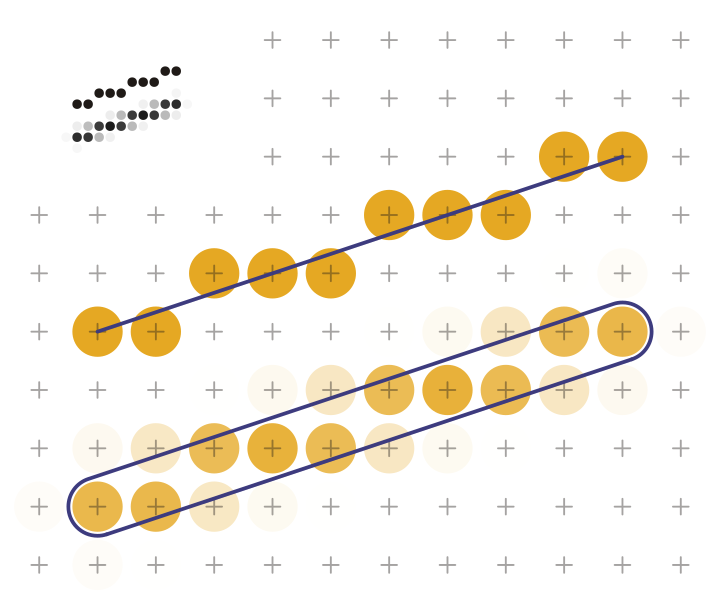
\includegraphics[width=0.4\textwidth]{slides/graphics-theory-pixel-drawing/line-sub-pixel-rendering.pdf}\\
  \textit{\small Pixel drawing versus sub-pixel drawing (x-axis major)}
  \end{center}
\end{frame}

\begin{frame}{Circles and polar coordinates}
  \begin{itemize}
  \item Circles centered on \((x_c,y_c)\) are defined (Pythagoras theorem) as:
\[
(x - x_c)^2+(y - y_c)^2 = radius^2
\]
  \end{itemize}
  \begin{minipage}{0.70\textwidth}
  \begin{itemize}
  \item Which is always verified with the expression:
\begin{gather*}
x = x_c + radius \times cos(\phi)\\
y = y_c + radius \times sin(\phi)
\end{gather*}
  \item Corresponds to a translation in polar coordinates
    \begin{itemize}
    \item From a \((x,y)\) base to \((r,\phi)\)
    \end{itemize}
  \item Iteration on \(\phi\) with a specific range: \(\phi \in [0;2\pi]\)
  \end{itemize}
  \end{minipage}
  \hfill
  \begin{minipage}{0.25\textwidth}
    \centering
    \includegraphics[width=0.8\textwidth]{slides/graphics-theory-pixel-drawing/polar-coordinates.pdf}
  \end{minipage}
\end{frame}

\begin{frame}{Parametric curves}
  \begin{itemize}
  \item Parametric curves generalize the idea of using independent parameters
  \item Each curve has defining equations and ranges for parameters
    \begin{itemize}
    \item Equations allow calculating \((x,y)\) (or \((r,\phi)\))
    \end{itemize}
  \item Drawing is achieved by iterating over parameter values
    \begin{itemize}
    \item Sampling is done on the range to get a finite number of points
    \item X/Y coordinates are calculated for each point
    \item Line interpolation is used between consecutive points
    \end{itemize}
  \item Ellipse: \(\phi \in [0;2\pi]\)
\begin{gather*}
x = x_c + a \times cos(\phi)\\
y = y_c + b \times sin(\phi)
\end{gather*}
  \item Many more parametric curves exist:
    \begin{itemize}
    \item Cycloid, Epicycloid, Epitrochoid, Hypocycloid, Hypotrochoid (spirograph)
    \item Lissajous Curve, Rose curve, Butterfly curve
    \end{itemize}
  \end{itemize}
\end{frame}
